 %% Simplified vision for Ausarbeitungen
\documentclass[%
paper=a4,      % alle weiteren Papierformat einstellbar
fontsize=11pt, % Schriftgr��e (12pt, 11pt (Standard))
BCOR1cm,       % Bindekorrektur, bspw. 1 cm
DIV15,         % f�hrt die Satzspiegelberechnung neu aus s. scrguide 2.4
%twoside,       % Doppelseiten
headsepline,   %
headings=openright, % Kapitel nur rechts beginnen
%biblography=totoc, % Literaturverzeichnis einf�gen bibtotocnumbered: nummeriert
parskip=half,  % Europ�ischer Satz mit Abstand zwischen Abs�tzen
chapterprefix, % Kapitel anschreiben als Kapitel
headsepline,   % Linie nach Kopfzeile
titlepage,     %
numbers=noenddot,
%draft	       % zeigt �berlange Zeilen an
]{scrreprt}

\usepackage{pdfpages}       % Titelseite hat ein anderes Layout. Sie wird 
                            % separat erzeugt und hier eingef�gt
\usepackage[T1]{fontenc}
\usepackage[utf8]{inputenc}  % Zeichencodierung
\usepackage[english]{babel} % Worttrennung nach neuer Rechtschreibung


\usepackage{siunitx}
\usepackage{ellipsis}       % Leerraum um Auslassungspunkte
\usepackage{fixltx2e}       % Fehlerkorrektur Zeichens�tze
\usepackage{xspace}         % f�ge evtl. notwendiges Leerzeichen hinzu (\xspace)
\usepackage{textcomp}
\usepackage{bm}

%\usepackage{mathptmx}           % Times + passende Mathefonts
\usepackage{mathpazo}           % Palatino + passende Mathefonts
\usepackage[scaled=.92]{helvet} % skalierte Helvetica als \sfdefault
\usepackage{courier}            % Courier als \ttdefault

\usepackage{graphicx}    % Einbindung von Grafiken
\graphicspath{{Images/}} % Unterverzeichnis, in dem Grafiken abgelegt werden
\usepackage{listings}    % Listenausgabe externer Dateien
\lstset{language=Matlab}
% \usepackage[framed,numbered,autolinebreaks,useliterate]{mcode}

\usepackage{float}      % Paket zum Erweitern der Floatumgebungen
\usepackage[figuresright]{rotating}   % Rotieren von Objekten
%\usepackage{hvfloat}
\usepackage{array}      % Paket zum Erweitern der Tabelleneigenschaften
\usepackage{booktabs}   % Paket f�r sch�nere Tabellen

\usepackage{amsmath}    % erweiterte Mathematik-Umgebungen
\usepackage{amssymb}
\usepackage{url}
\usepackage{subfigure}



% Einstellungen f�r das Literaturverzeichnis
\usepackage[round]{natbib}
\setlength{\bibsep}{0.5\baselineskip}
\setlength{\bibhang}{1cm}
\bibliographystyle{agsm}

% Andere Schriftarten in Koma-Script
\setkomafont{sectioning}{\normalfont\bfseries}
\setkomafont{captionlabel}{\rmfamily\bfseries\small}
\setkomafont{caption}{\mdseries\itshape\small}
\setkomafont{pagehead}{\normalfont\itshape} % Kopfzeilenschrift
\setkomafont{descriptionlabel}{\normalfont\bfseries}

% Kopf und Fu�zeilen
\usepackage[automark]{scrlayer-scrpage}

% Hyperref
\usepackage{hyperref}

% Literaturverzeichnis-Stil
\bibliographystyle{plain}

% weitere Einstellungen
\tolerance=200               % �bervolle Zeile vermeiden
\emergencystretch=3em

\clubpenalty=10000           % 'Schusterjungen' und 'Hurenkinder' vermeiden
\widowpenalty=10000 
\displaywidowpenalty=10000

\parindent 0pt               % Einzug zu Absatzbeginn festlegen

\setcapindent{1em}           % Zeilenumbruch bei Bildbeschreibungen.

\setcounter{secnumdepth}{3}  % Strukturiertiefe bis subsubsection{} m�glich
\setcounter{tocdepth}{3}     % Dargestellte Strukturiertiefe im Inhaltsverzeichnis

% Korrekturversion mit 1.5-fachem Zeilenabstand im Hauptteil:
\newif\ifiscorrect
%\iscorrecttrue   % Korrekturversion
\iscorrectfalse % keine Korrekturversion

%% Eigene Definitionen:

% Einheiten:
\def\ut#1{\ensuremath{\,\mathrm{#1}}}

% Operatoren:
\def\grad{\ensuremath{\mathop{\mathrm{grad}}\nolimits}}
\def\transp#1{\ensuremath{{#1}^\mathsf{T}}}  % transpose
\def\const{\ensuremath{\mathop{\mathrm{const.}}\nolimits}}

% Formelzeichen:
\def\vec#1{\ensuremath{\mathbf{#1}}}
\def\matr#1{\ensuremath{\mathbf{#1}}}

% Hack, um ein zus�tzliches Leerzeichen nach \input zu entfernen:
\def\myinput#1{%
  \endlinechar=-1 % kein Zeilenabschlusszeichen
  \input #1\relax
  \endlinechar `\^^M % Zeilenabschluss = Zeilenvorschub
}



\begin{document}
\selectlanguage{ngerman}
\pagenumbering{Roman}
\pagestyle{plain}

%% Title

\includepdf[pages=1]{title}

%% Table of contents
\pagestyle{scrheadings}
\clearscrheadfoot            % Standardkram wegwerfen
\ohead[\pagemark]{\pagemark} % oben au�en Seitenzahl 
%% Ausarbeitung简化版目录,只保留内容目录
\tableofcontents
\clearpage

% Pages number: roemisch
% Nmber in the text: arabic
\newcounter{roemisch}
\setcounter{roemisch}{\value{page}}
\pagenumbering{arabic}

\ifiscorrect\linespread{1.5}\selectfont % ???: 1 1/2 (f�r bessere Korrektur)
\else\fi

%% Chapters
% Kopfzeile: links Kapitel, rechts Sektion
\clearscrheadfoot            % Standardkram wegwerfen
\ohead[\pagemark]{\pagemark} % oben au�en Seitenzahl 
\ihead{\headmark}            % oben innen automatischer Abschnittsname
\automark[]{section}
\chapter{Report}
\section{Introduction}
The A-0-A method is a new approach for correcting drift in seafloor pressure measurement. In this work 2 A-0-A calibrated pressure gauges and a three-component accelerometer were set on the MARS cabled observatory in Monterey Bay and 30-months data were collected.


\section{A-0-A Correction}
A total of 154 A-0-A calibrations were performed with each lasting 5 minutes, an Example is shown in \autoref{fig:A0Aexample}, The measured pressure drop initially overshoots to pressure lower than atmospheric because of short term viscoelastic transients and because the adiabatic expansion of oil leads to cooling that takes some time to equilibrate. After removing the first and last 30 seconds, the mean value of difference. In this example, $mean(P_{1,int} - baro) = 1.14 \ut{hpa}$ and $mean(P_{2,int} - baro) = -1.19 \ut{hpa}$  
\begin{figure}[htpb]\centering
	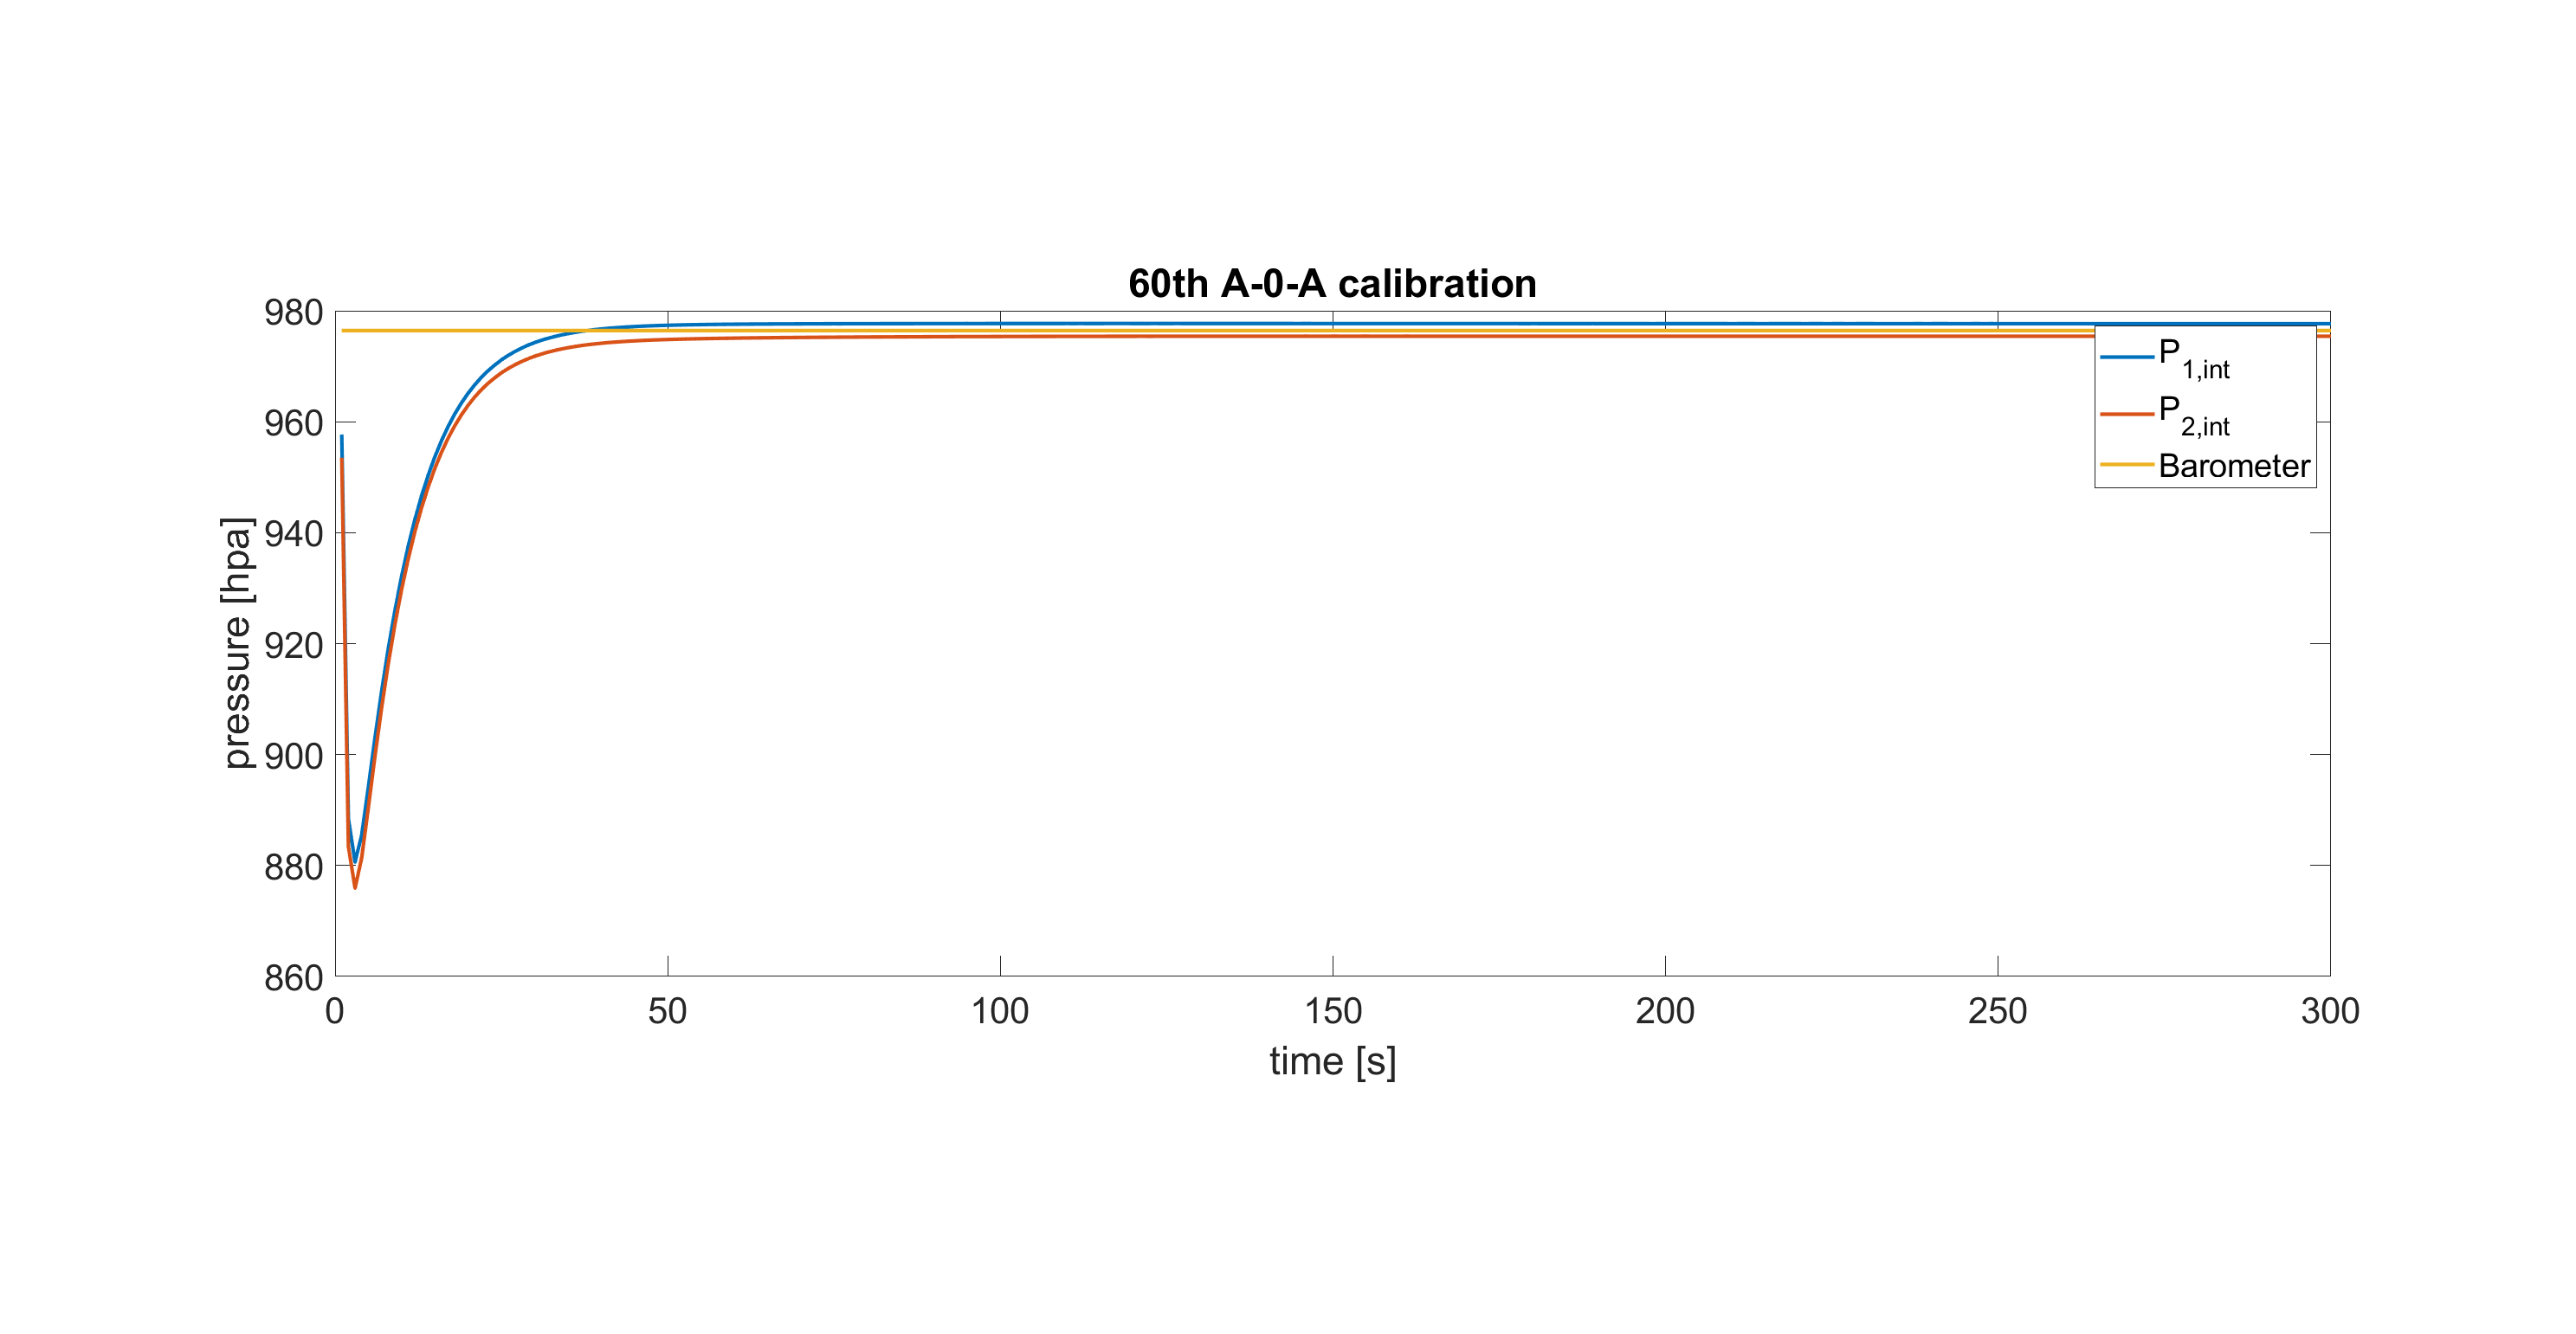
\includegraphics[width=0.9\textwidth]{calibrationExample.png}
	\caption{Example A-0-A Calibration}
	\label{fig:A0Aexample}
\end{figure}\\
The results of all calibrations are in \autoref{fig:A0A}
\begin{figure}[htpb]\centering
	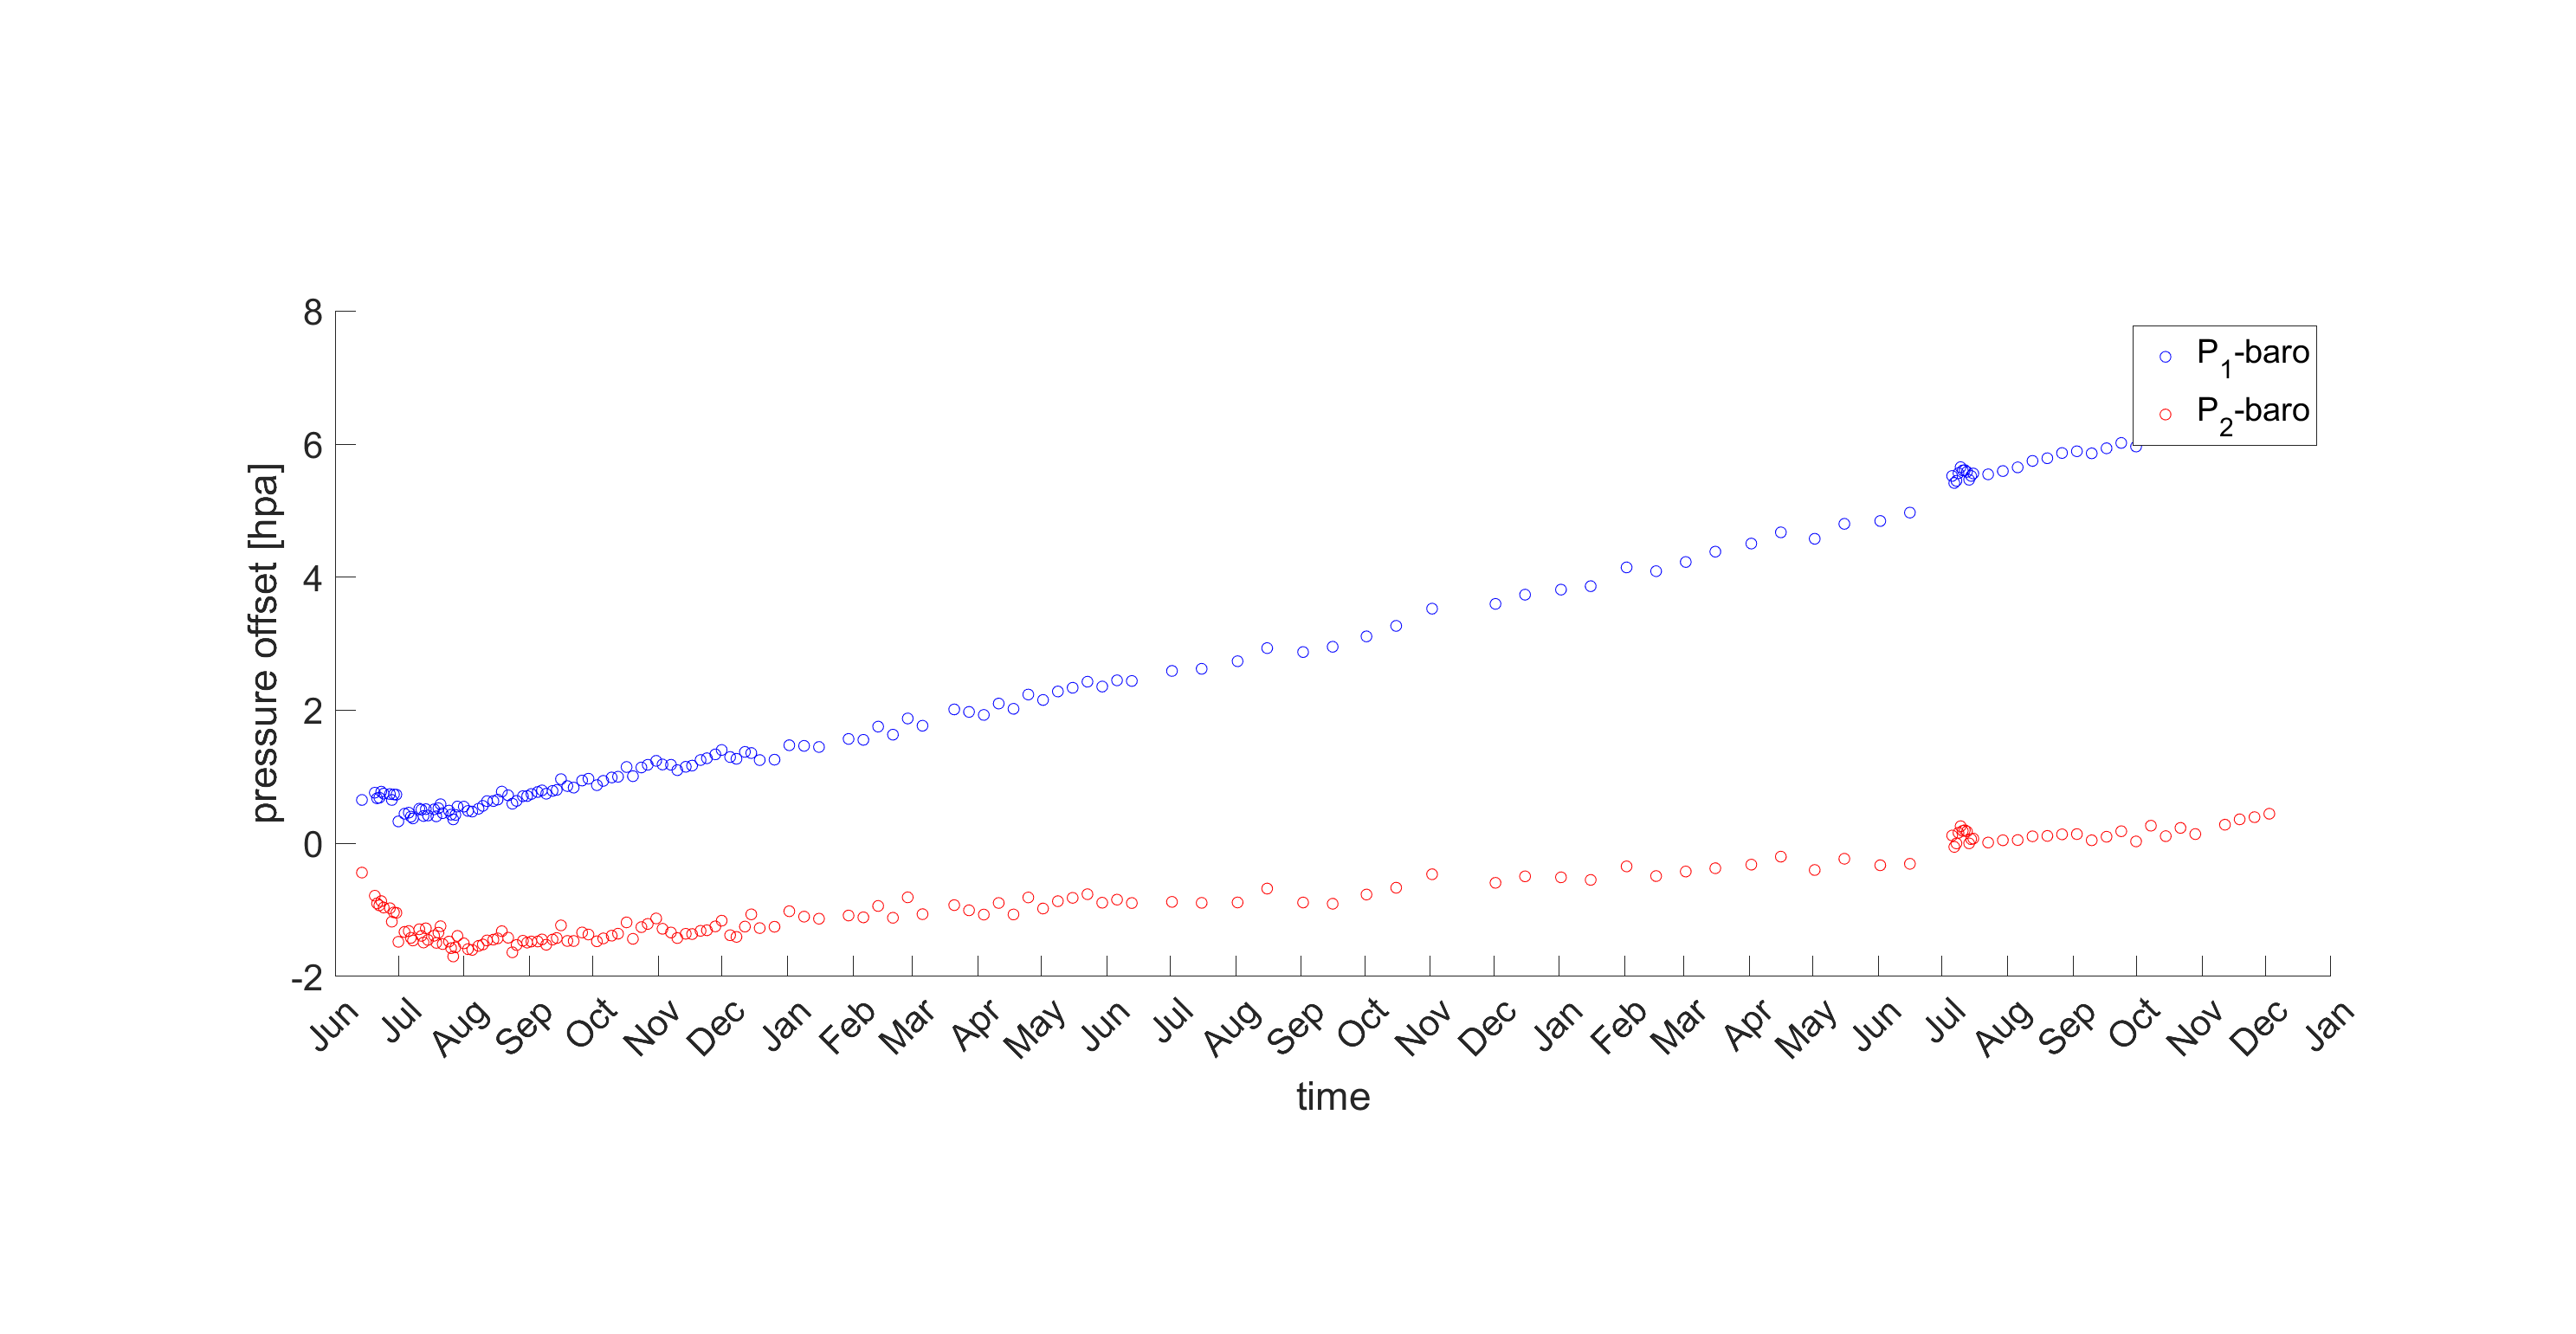
\includegraphics[width=0.9\textwidth]{a0a.png}
	\caption{Result A-0-A Calibration}
	\label{fig:A0A}
\end{figure}\\
This series follow a form of function
\begin{equation}
	p(t) = a \cdot exp(-t/t_0) + bt + c + d(T-T_{ref})
\end{equation}
Where $a$,$b$,$c$,$d$ and $t_0$ are the parameters. $t_0$ is a time constant since the deployment which gives the minimum RMS. After a iteration, $t_0 = 351 \ut{day}$ for gauge 1 and $t_0 = 759 \ut{day}$ for gauge 2. A Least square will be implemented to get 2 parameters groups for gauge 1 and 2. $T$ is the Temperature and $T_{ref}$ the reference temperature which is here the median temperature since the deployment. A smoothing line is in \autoref{fig:smoothing}. Then, this calibration can be used for the whole datasets. 
\begin{figure}[htpb]\centering
	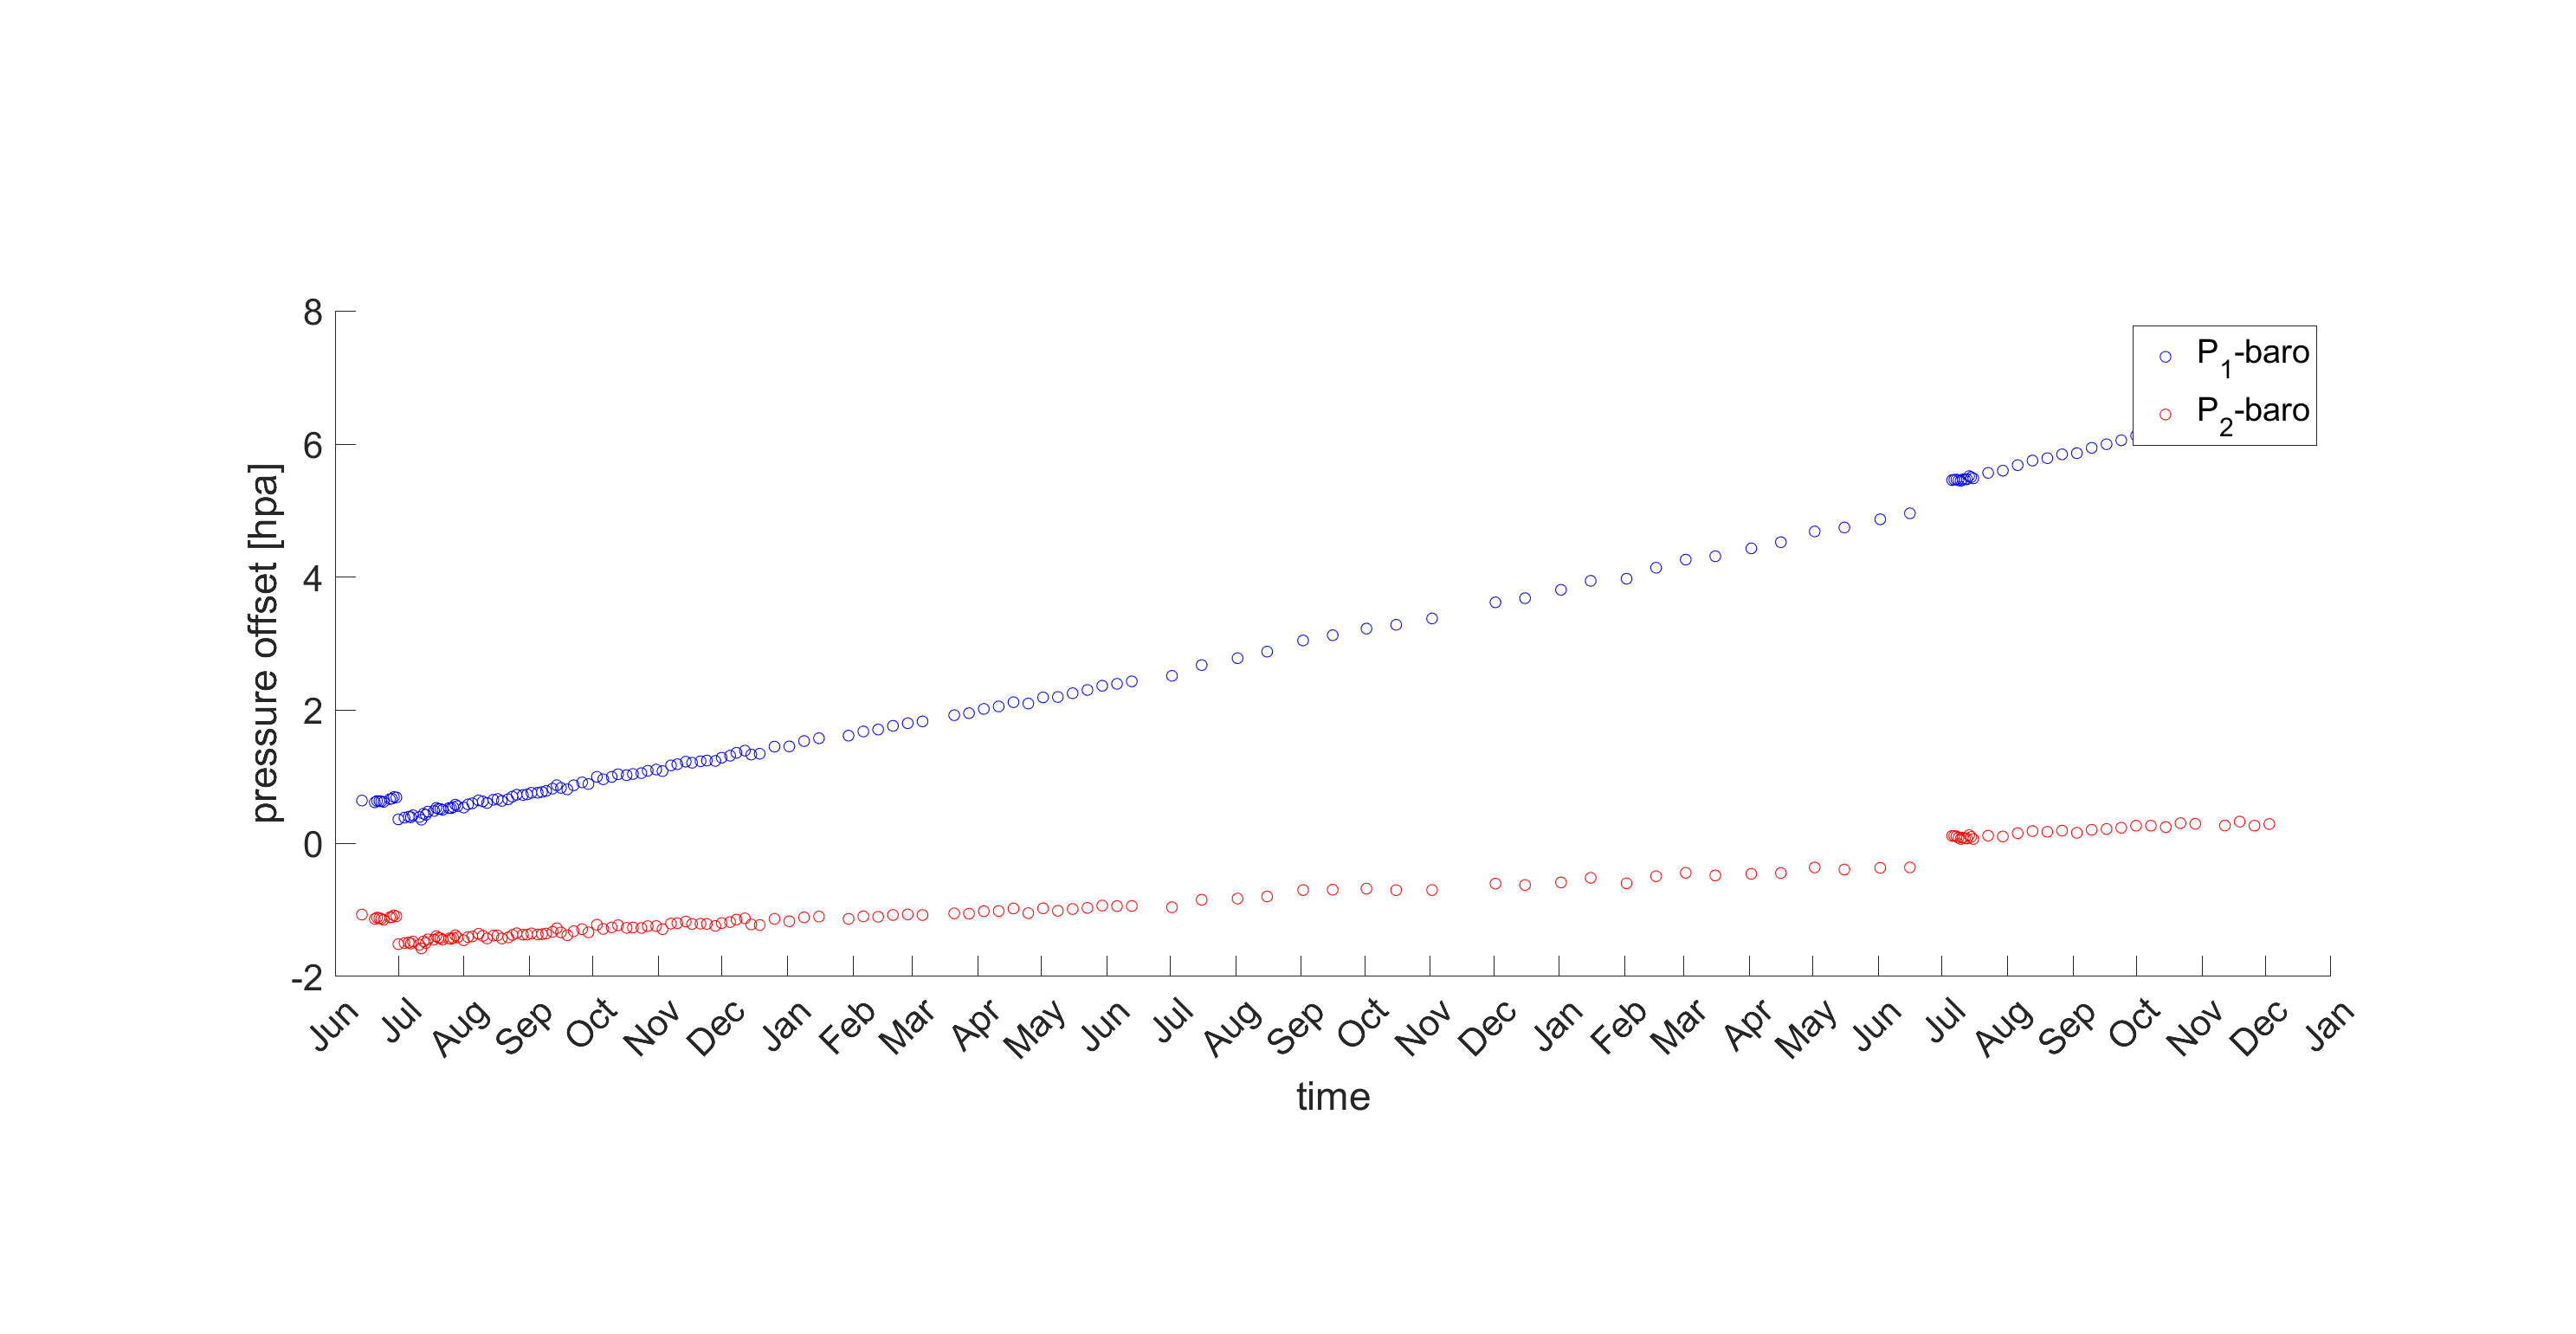
\includegraphics[width=0.9\textwidth]{smoothing.png}
	\caption{calibration model}
	\label{fig:smoothing}
\end{figure}


\section{Data}
The measurements took place every 1 minutes, \autoref{fig:examplePressure} shows a part of result in 10.Aug.2017. It is obvious that the pressure varies due to diurnal and semi-diurnal tides, but the difference between them remains stable.
\begin{figure}[htpb]\centering
	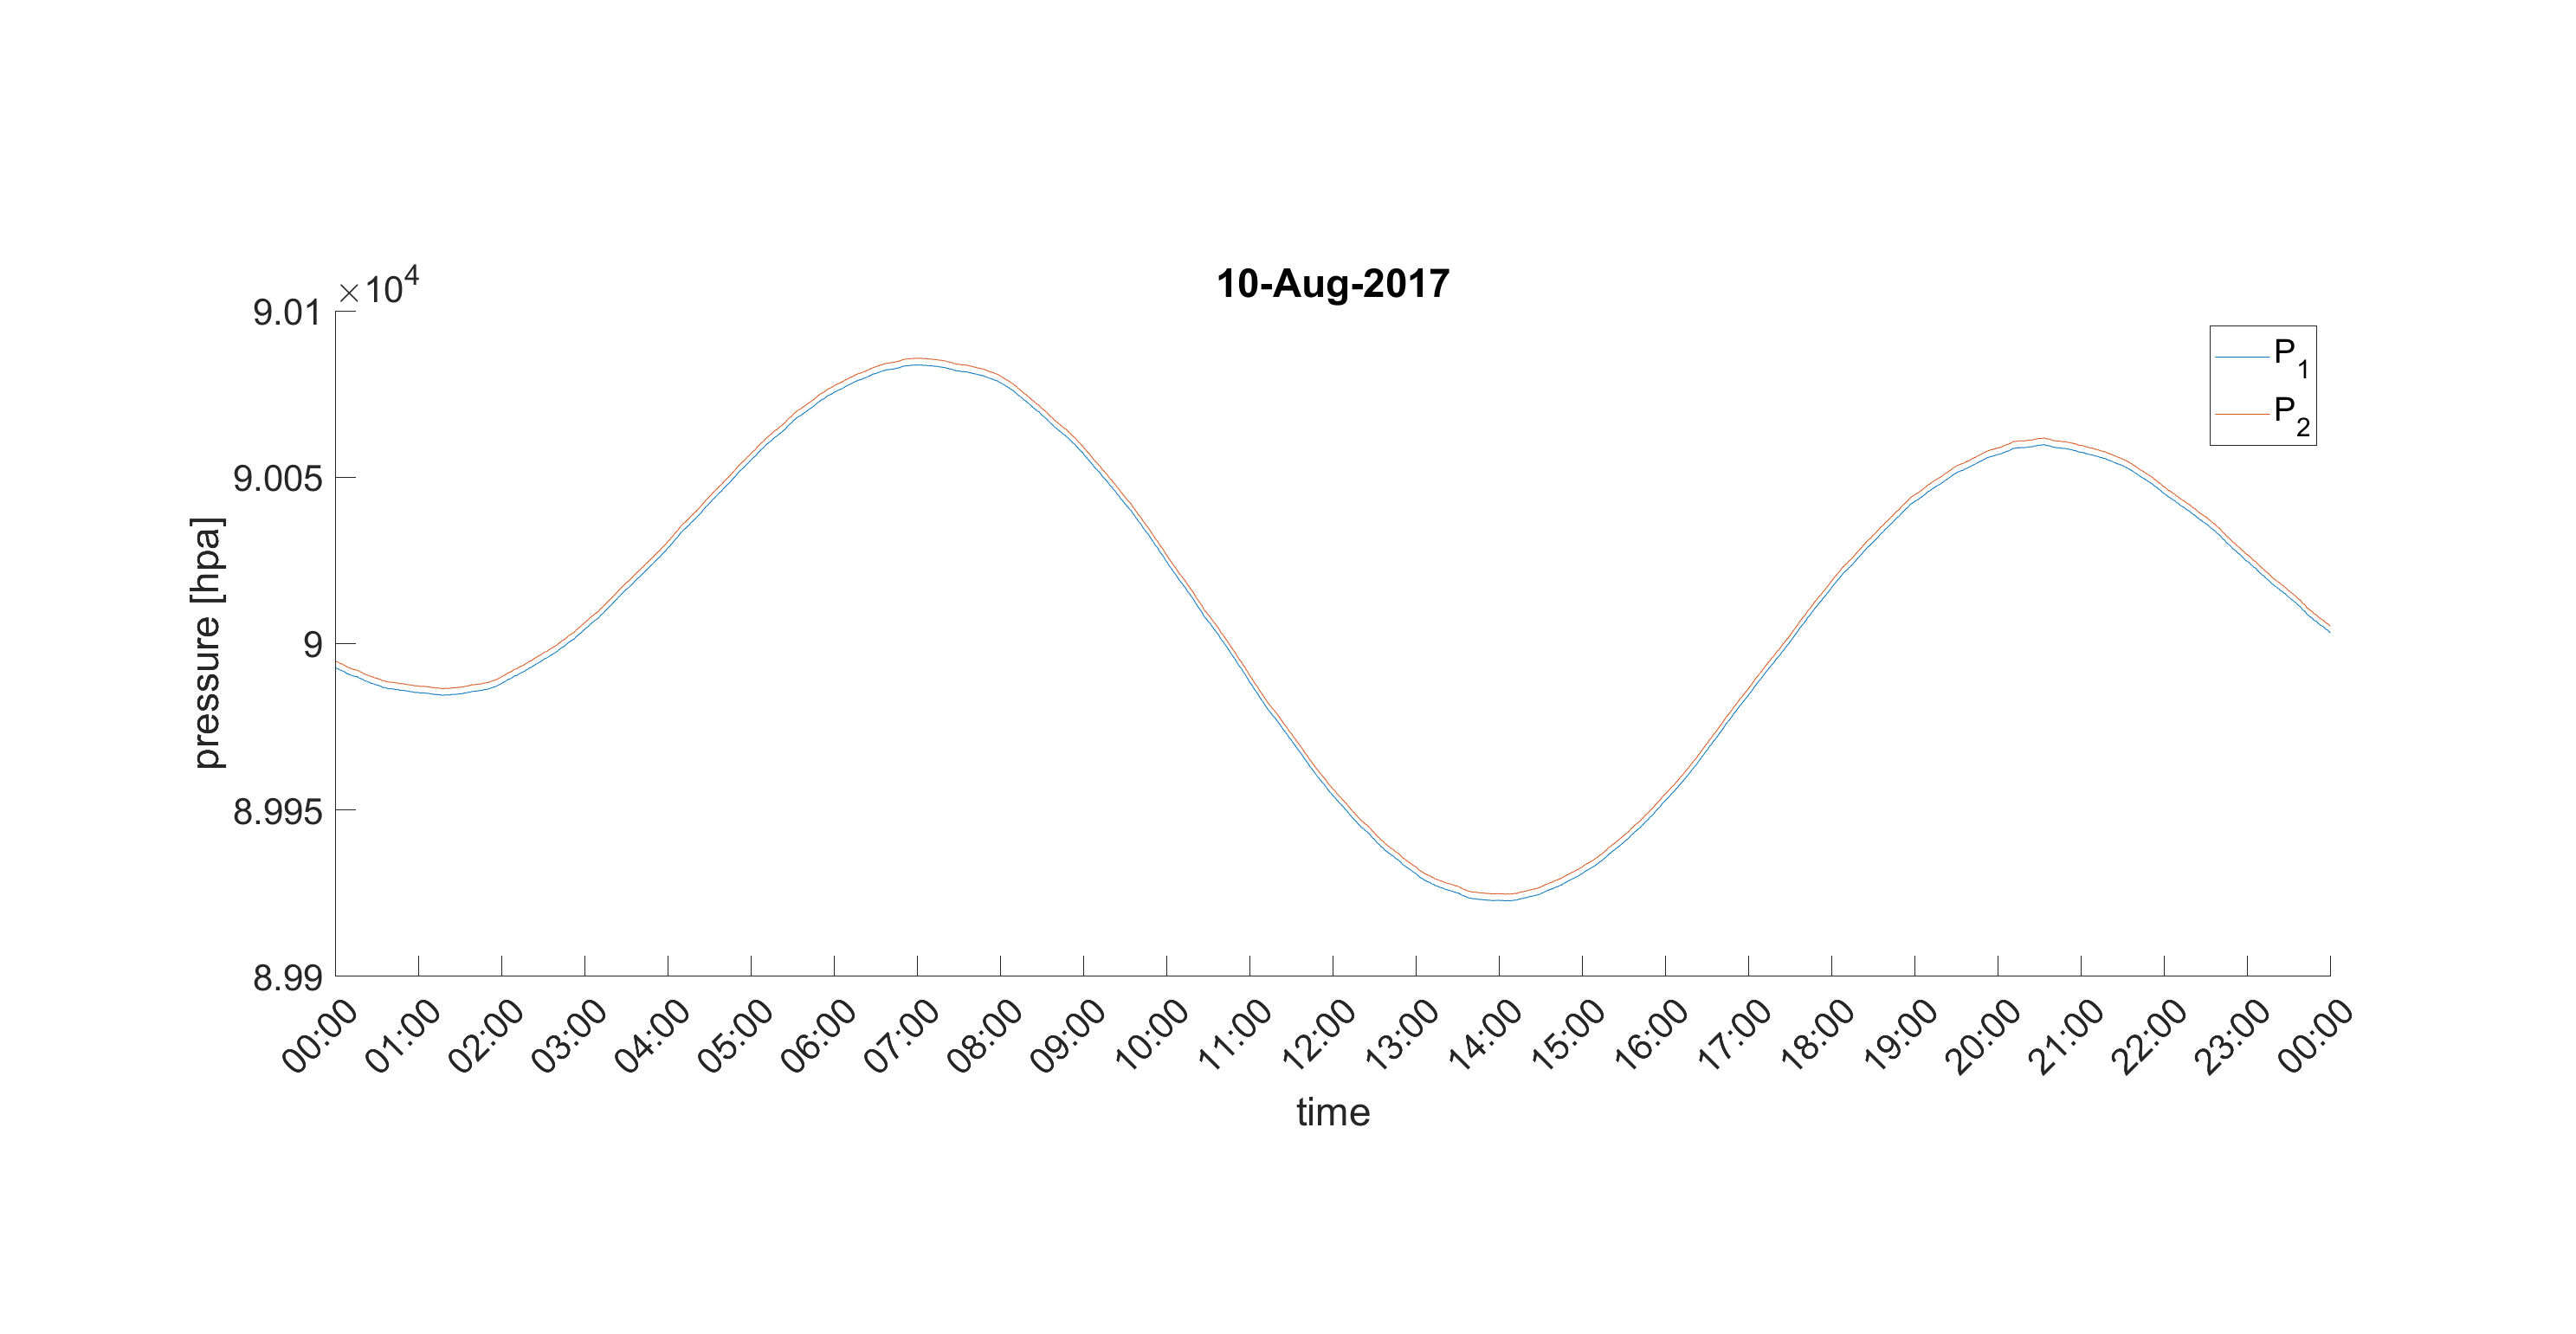
\includegraphics[width=0.9\textwidth]{examplePressure.png}
	\caption{Pressure in 10.Aug.2017}
	\label{fig:examplePressure}
\end{figure}\\\\
Therefor, the daily mean pressure will be calculated. We noticed that there are several gaps in the whole time series, if this gap is too big and can't be interpolated, the data of this day shall not be used. In the end, the results are shown in \autoref{fig:pressure}. 
\begin{figure}[htpb]\centering
	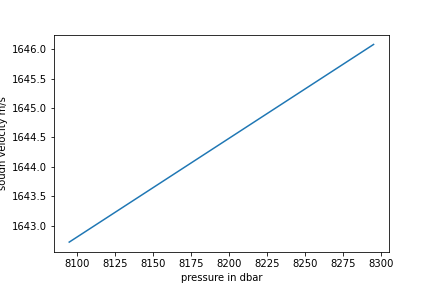
\includegraphics[width=0.9\textwidth]{pressure.png}
	\caption{Pressure}
	\label{fig:pressure}
\end{figure}\\\\
The Trend of two time series is $0.732 \ut{hpa/year}$ for gauge 1 and $0.686 \ut{hpa/year}$. The difference between two time series are very stable after calibration. 



\section{Tilt}
The platform tilt has been not taken into consideration till now, \autoref{fig:acceleration} shows the change in accelerator mearsuments over deployment, and so the tilt can be calculated (\autoref{fig:tilt}).
\begin{align}
	tilt = & \frac{a_{horizontal}}{a_{vertical}} \\
	     = & \frac{\sqrt{a_y^2 + a_z^2}}{a_x}
\end{align}
By Analysing the shape of the platform\autoref{fig:plat}, we can estimate a subsidence of one leg by nearly 1 cm of the observed tilt. To remove this effect, we remove external pressure over the experiment by 0.3 hpa.
\begin{figure}[htpb]\centering
	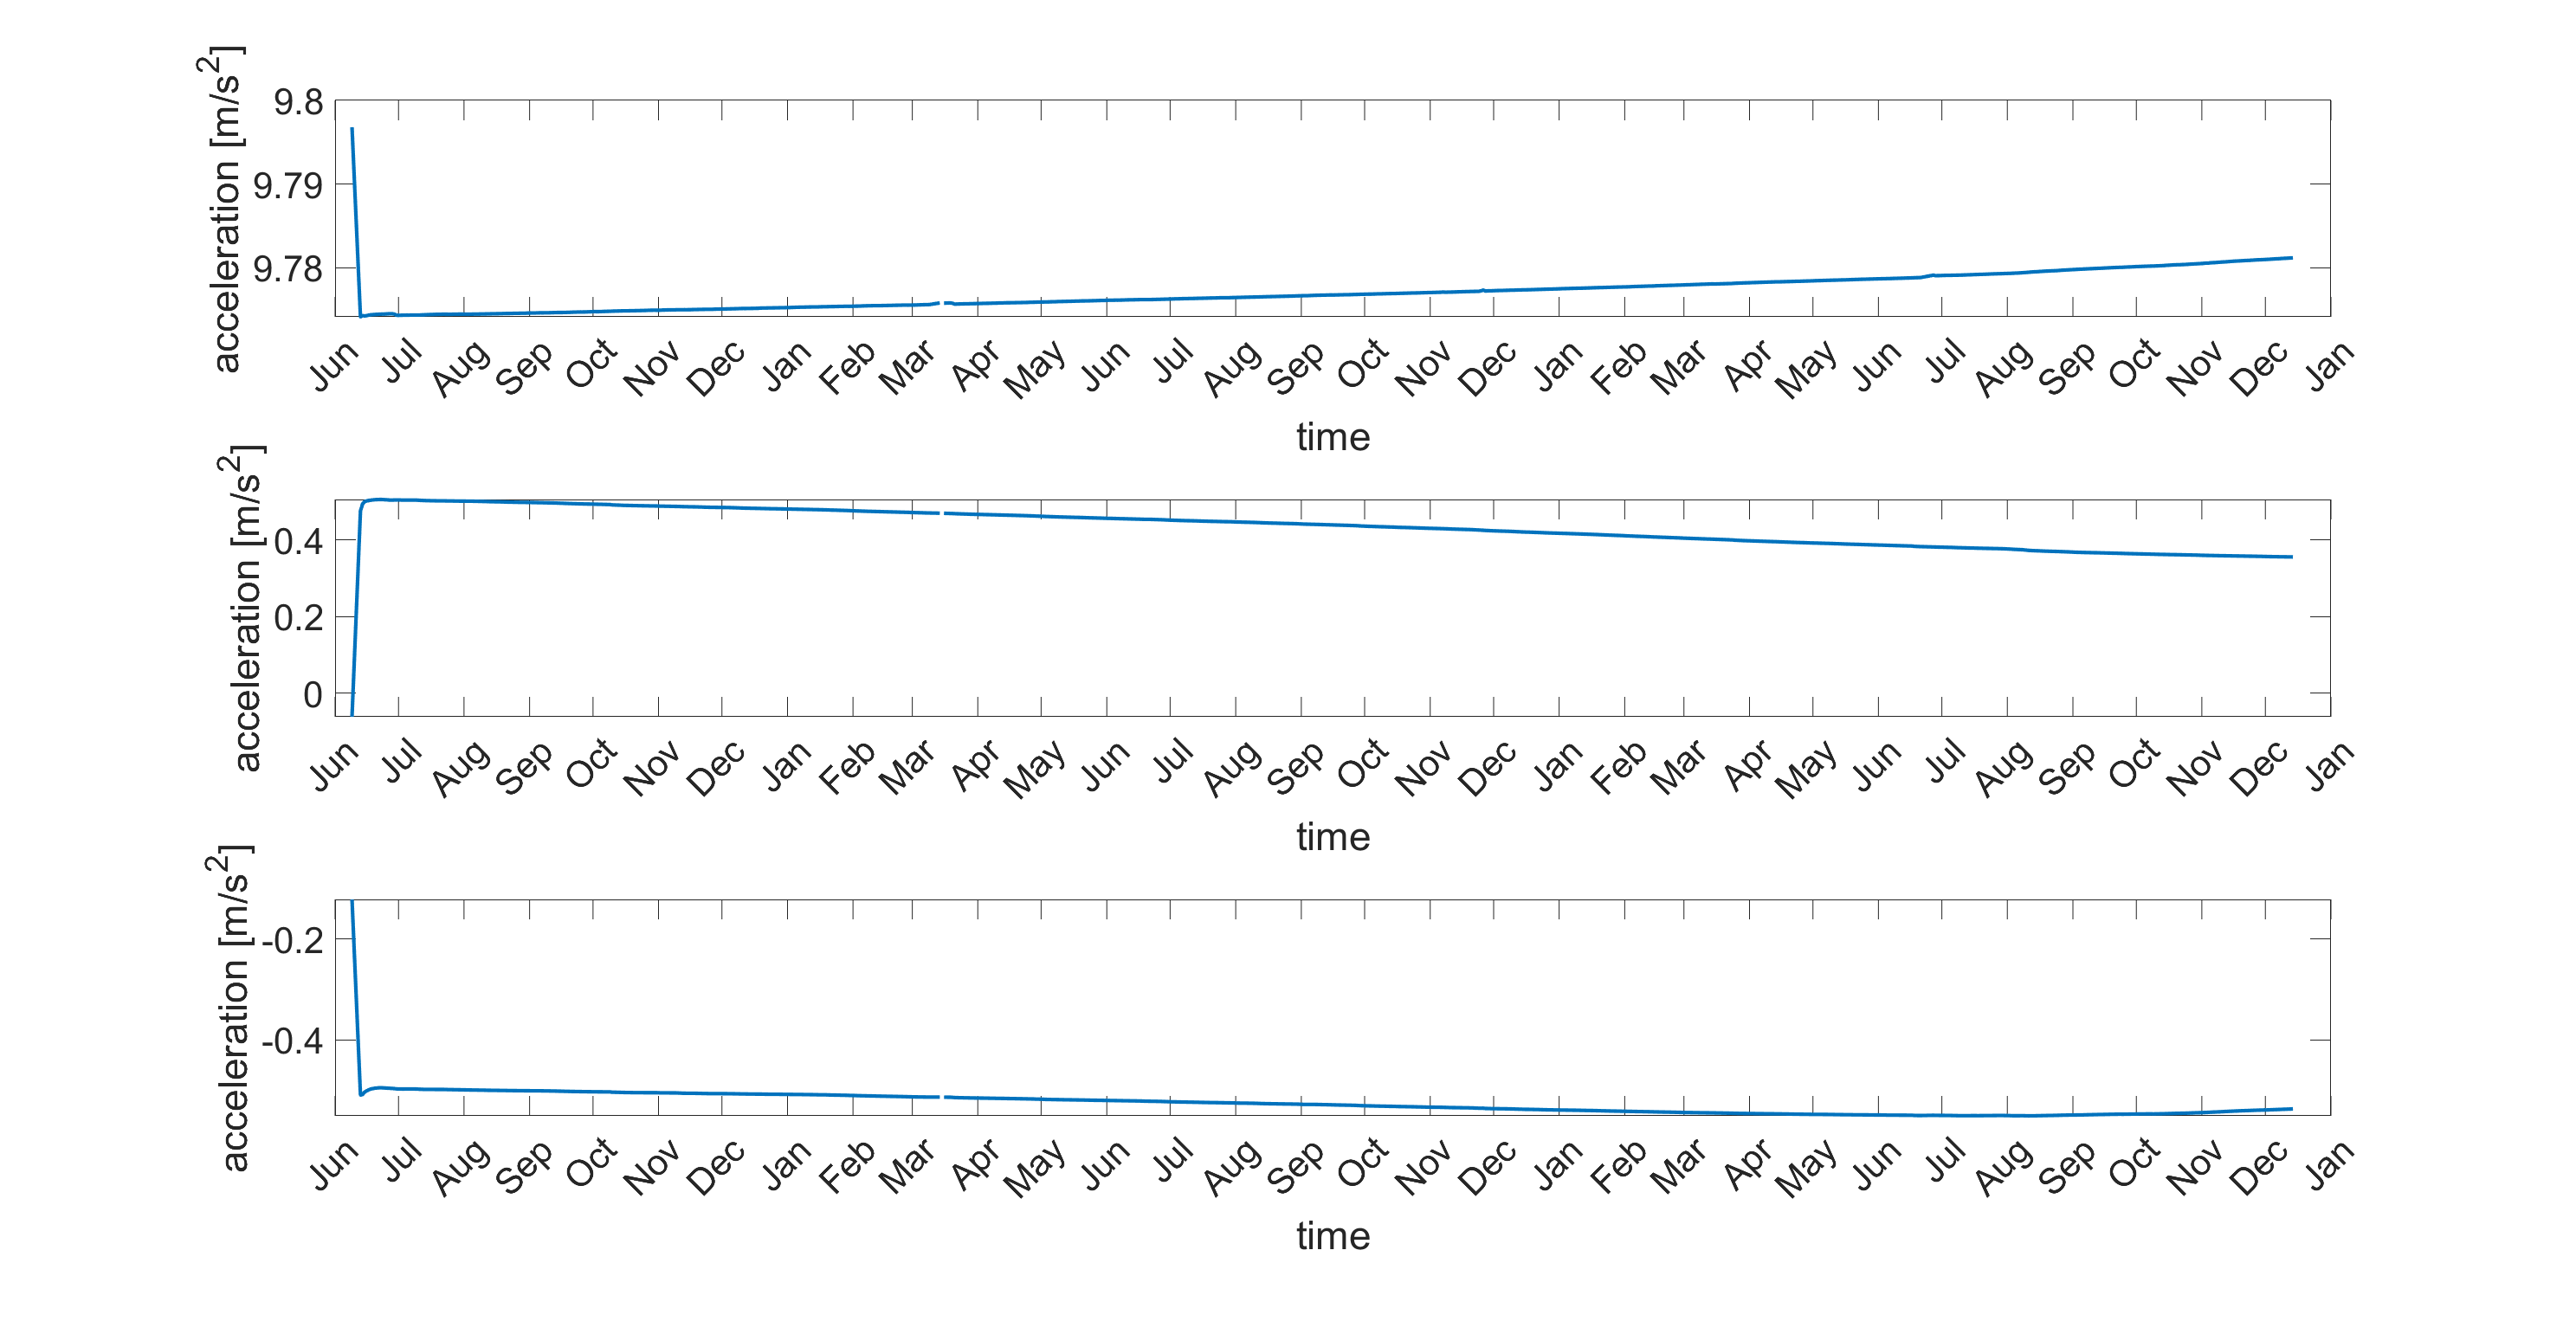
\includegraphics[width=0.9\textwidth]{acceleration.png}
	\caption{Acceleration}
	\label{fig:acceleration}
\end{figure}
\begin{figure}[htpb]\centering
	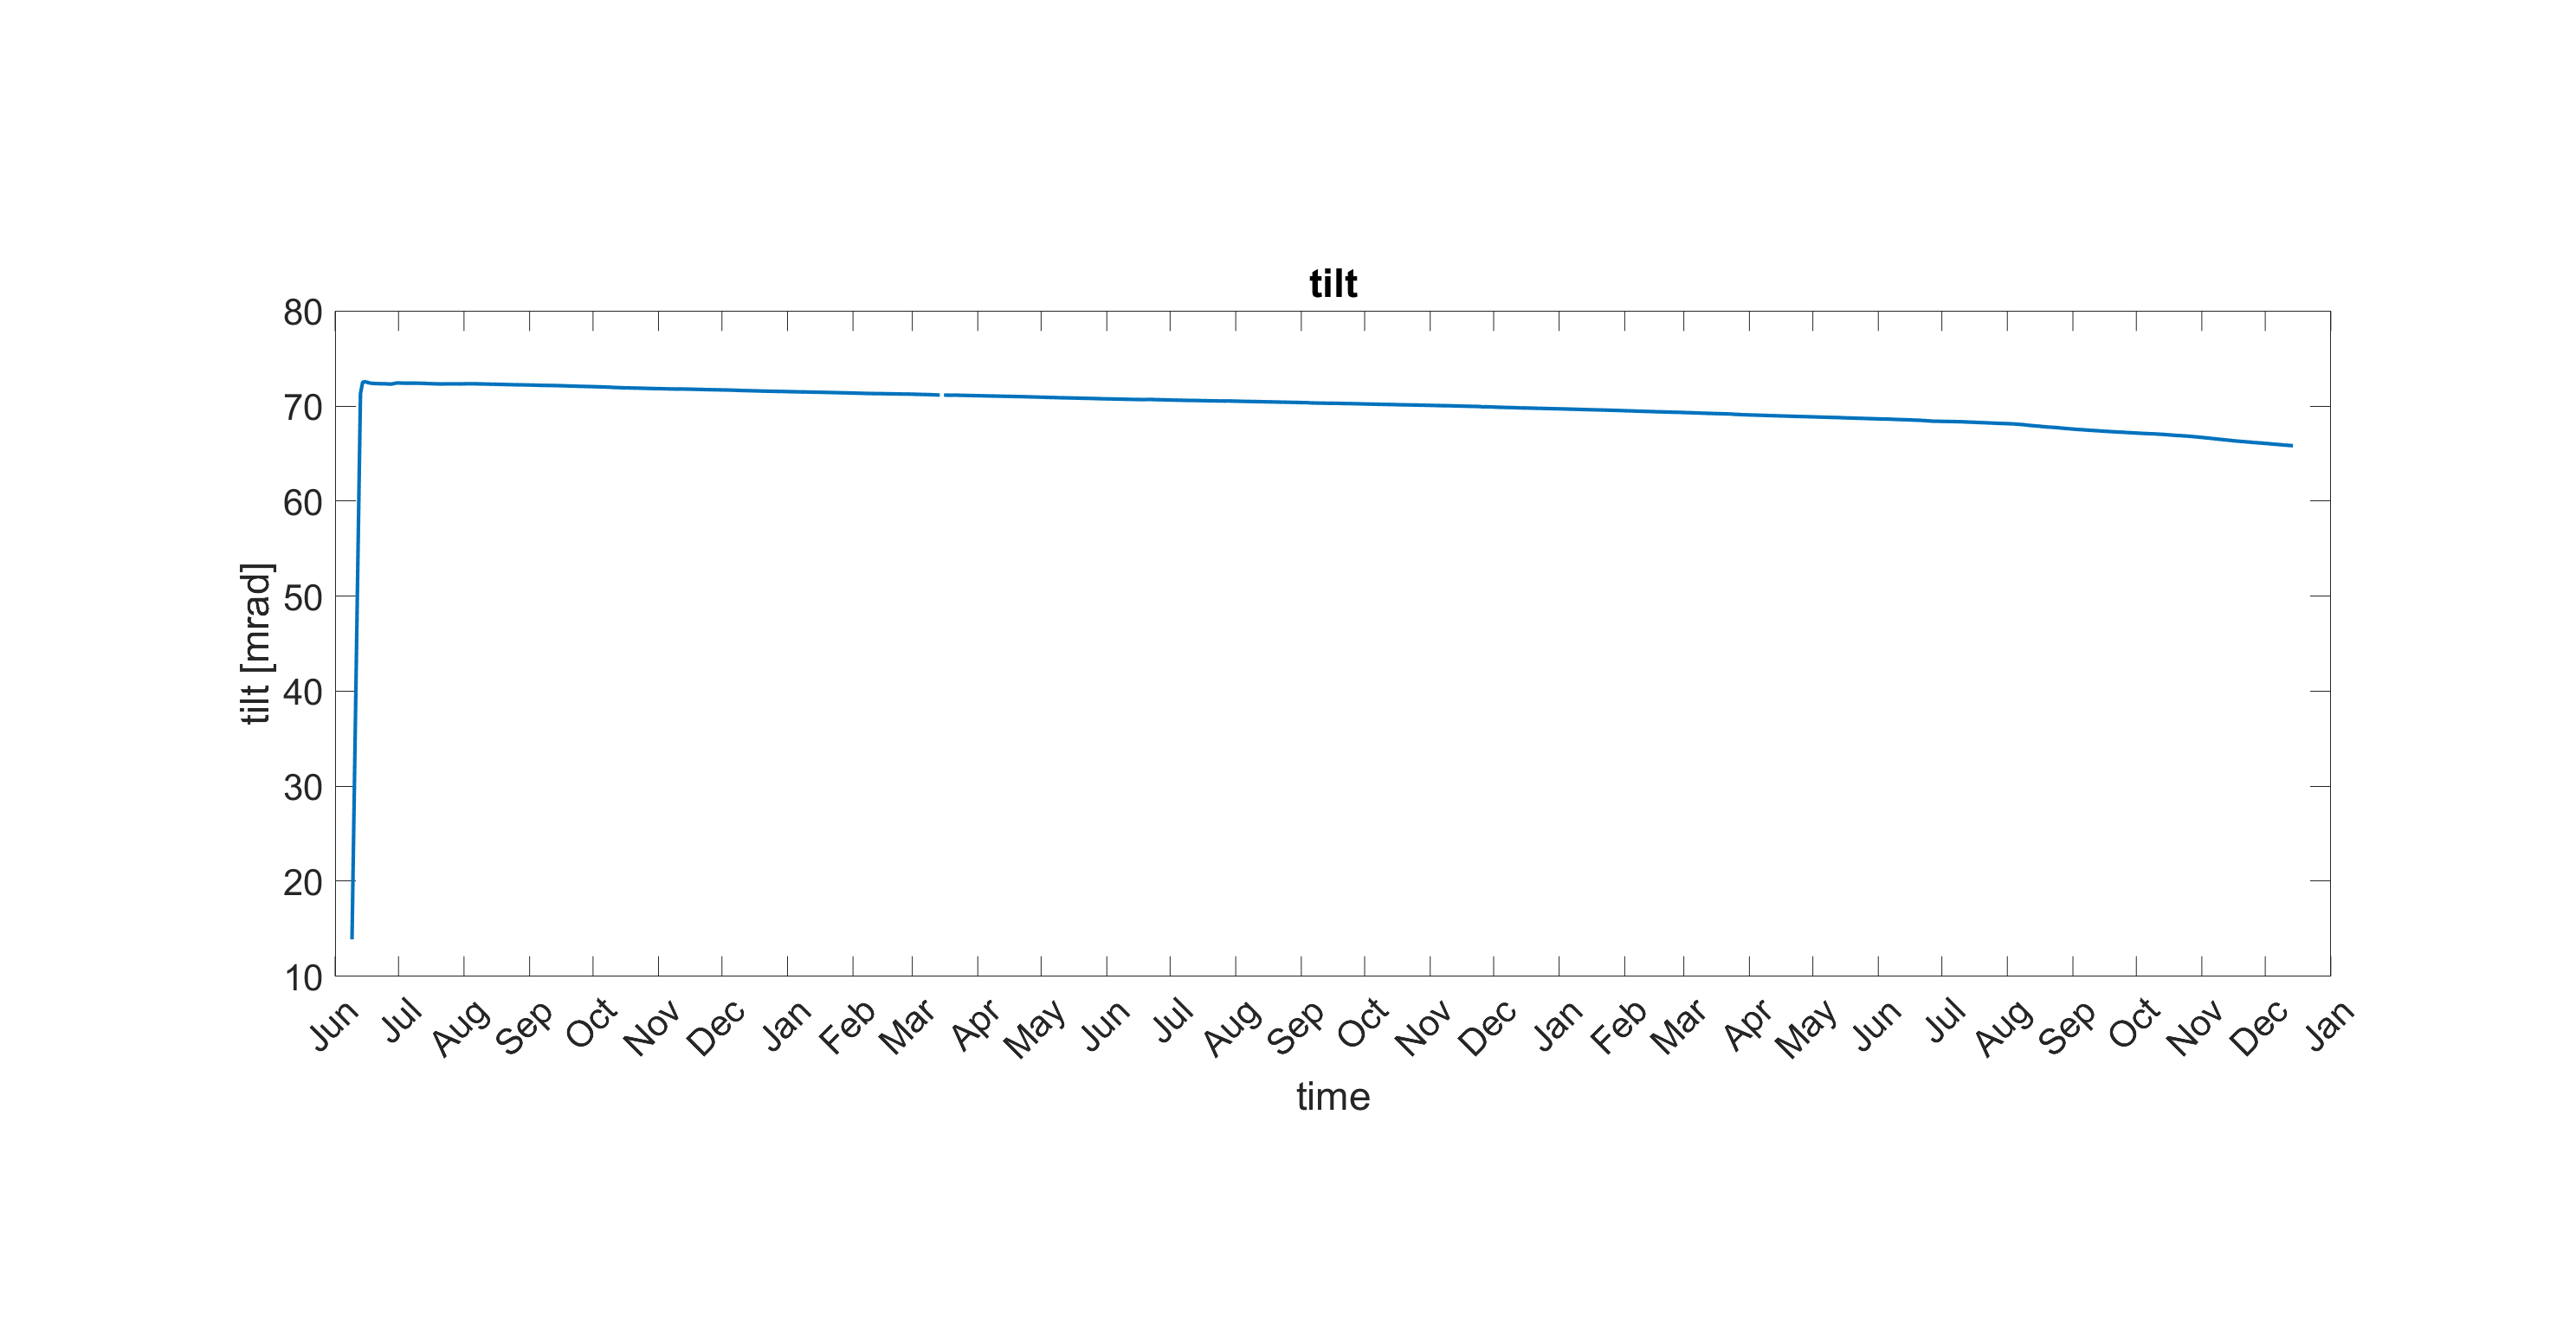
\includegraphics[width=0.9\textwidth]{tilt.png}
	\caption{Tilt}
	\label{fig:tilt}
\end{figure}
\begin{figure}[htpb]\centering
	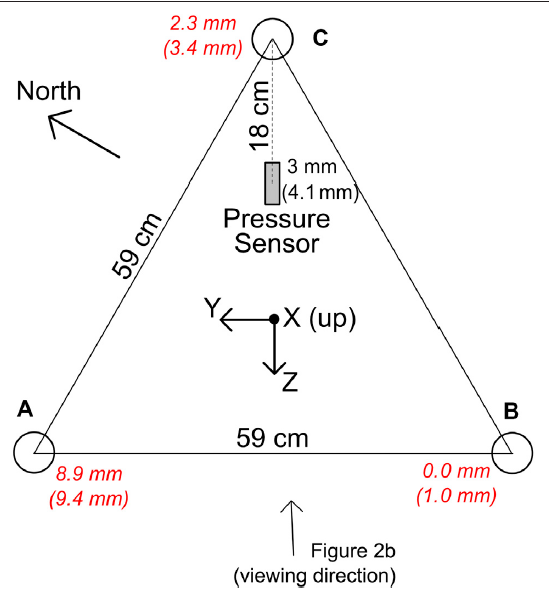
\includegraphics[width=0.6\textwidth]{platform.png}
	\caption{Platform}
	\label{fig:plat}
\end{figure}



\section{Another Effects}
According to the paper, the tide influences should be excluded from the pressure measurements. This was done in the paper using low-pass Godin filter, which remains unclear. Therefor, this step was not performed in this work.\\\\
There are other error sources, which is the combined effects of changes in oil reservoir level, counting clock drift and the minimum subsidence. The correction is set to 0.1 hpa. 



\section{Discussion}
This trend of increasing pressure are consistent with the trend with the trend expected from the El Niño Southern Oscillation. This effect is not a result of density structure but is related partly to variations in local wind stress moving water toward or away from the coast and partly due to the effects of coast trapped waves generated by wind stresses elsewhere. \cite{ryan2002sea}. The first winter of the GSSM deployment coincided with weak La Niña event from October 2017-March 2018 while the latter parts of the deployment coincided with weak El Niñoconditions from October 2018-June 2109 and Novenmber-December 2019.


\ifiscorrect\linespread{1.0}\selectfont% Zeilenabstand wieder auf 1 zur�ck
\else\fi

% Setze Numerierung wieder auf r�misch zur�ck und setzte von oben fort
% Wert ist demnach der von 'roemisch'
\newpage
\pagenumbering{Roman}
\setcounter{page}{\value{roemisch}}


\end{document}
